\section{Intervals, Regions, Open and Closed Sets}
\textit{Lecture 3 (Sept 15)}
\begin{itemize}
    \item In single-variable calculus, we typically focused on an interval $[a,b]$ on the real number line. Similarly, we can talk about intervals in $\mathbb{R}^2$ which can be represented as a rectangle:
          \begin{center}
              \begin{tikzpicture}
                  \draw[->] (0,0) -- (6,0) node[right] {$x_1$};
                  \draw[->] (0,0) -- (0,5) node[right] {$x_2$};

                  \draw[draw=black] (2,2) rectangle ++(3,2);
                  \draw[dotted] (2,2) -- (2,0) node[below] {$a_1$};
                  \draw[dotted] (5,2) -- (5,0) node[below] {$b_1$};
                  \draw[dotted] (2,2) -- (0,2) node[left] {$a_2$};
                  \draw[dotted] (2,4) -- (0,4) node[left] {$b_2$};

              \end{tikzpicture}
          \end{center}
    \item We can generalize to $\mathbb{R}^n$. Given $a_i \le b_i$ for $i=1,\dots,n$, we can define the \textbf{closed rectangle} corresponding to $a_i,b_i$:
          \begin{equation}
              R = \prod_{i=1}^n [a_i,b_i] = \{x\in \mathbb{R}^n: \forall i\, a_i \le x_i \le b_i\}
          \end{equation}
    \item Recall from set theory, if $X$ and $Y$ are sets, then $X \times Y = \{(x,y): x\in X, y\in Y\}$ (also referred to as direct product in group theory). This is associative (up to isomorphism), so
          \begin{equation}
              (X\times Y) \times Z \neq X \times (Y\times Z)
          \end{equation}
          but
          \begin{equation}
              (X\times Y) \times Z \cong X \times (Y\times Z).
          \end{equation}
          As a result, while they are not equal strictly speaking, we can view them as the same.
    \item We can then view $\mathbb{R}^n$ as
          \begin{equation}
              \mathbb{R}^n = \mathbb{R} \times \mathbb{R} \times \cdots \times \mathbb{R} = \{(x_1\,\dots\, x_n):x_i \in \mathbb{R}\}
          \end{equation}
    \item Products of intervals can be written as
          \begin{equation}
              \prod_{i=1}^n [a_i,b_i] = \{(x_1,\dots,x_n): \forall i\, x_i \in [a_i,b_i]\}
          \end{equation}
    \item Likewise, there are also \textbf{open rectangles.} Specifically, the open rectangle defined by $a_i,b_i$ is
          \begin{equation}
              \prod_{i=1}^n (a_i,b_i) = \{ (x_1,\dots,x_n) \forall i\, x_i \in (a_i,b_i)\}
          \end{equation}
    \item There is a way to define continuity using open sets.
          \begin{definition}
              The subset $A \subset \mathbb{R}^n$ is called ``open'' if:
              \vspace{2mm}

              For every $a\in A$, there exists an open rectangle $R$, such that $a\in R \subset A$.
          \end{definition}
          Note that this isn't the only definition. Instead of surrounding $a$ with a rectangle, we can surround $a$ with an open ball $B$ instead.
          \begin{definition}
              An open ball $B$ is a ball of radius $r$ centered at $x_0$:
              \begin{equation}
                  B = B_r(x_0)=\{y\in \mathbb{R}^n: |x_0-y| < r\}
              \end{equation}
          \end{definition}
          This implicitly gives rise to the theorem:
          \begin{theorem}
              Defining ``open'' sets using rectangles is equivalent to defining ``open'' sets using balls.
          \end{theorem}
          \begin{proof}
              The intuition of the proof is as follows:
              \begin{enumerate}
                  \item Suppose $A$ is open, so we can construct a rectangle $R$ around $a \in A.$
                  \item In the rectangle, we can find a ball $B$ such that $B \subset R$.
              \end{enumerate}
              This shows one direction of the proof. The other direction is as follows:
              \begin{enumerate}
                  \item Suppose $A$ is open, so we can construct a ball $B$ around $a\in A$.
                  \item In the ball, we can find a rectangle $R$ such that $R \subseteq B$.
              \end{enumerate}
              This is equivalent to showing that every open rectangle is open using the ball definition and that every open ball is open using the rectangle definition.
          \end{proof}
    \item Note that balls depend on the norms that we use. Norms in $L^1,L^2,L^\infty$ will all look different. We can use any of these norms to define a ball and still be valid in the theorem.
    \item We can also define closed sets.
          \begin{definition}
              $B$ is \textbf{closed} if $\mathbb{R}^n \setminus B = B^{C}$ is open.
          \end{definition}
          \begin{theorem}
              We have the following theorems related to open and closed sets.
              \begin{enumerate}
                  \item $\emptyset,\mathbb{R}^n$ are both closed and open.
                  \item Any union of open sets is open. Any intersection of closed sets is closed.
                  \item A finite intersection of open sets is open. A finite union of closed sets is closed.
              \end{enumerate}
          \end{theorem}
          \begin{proof}
              We prove each separately:
              \begin{enumerate}
                  \item To show that $\mathbb{R}^n$ is open, we just need to show that every point in $x\in\mathbb{R}^n$ is contained in a rectangle, i.e. $x\in \prod (x_i-1,x_i+1)\subset \mathbb{R}^n.$ This also implies that $\emptyset$ is closed.

                        To finish, we need to show that $\emptyset$ is open. Since there are no points in $\emptyset,$ the condition holds\footnote{This is analog to: Every horse in an empty set of horses has horns.}. This also implies that $\mathbb{R}^n$ is closed.
                  \item Suppose $\{A_\alpha\}_{\alpha \in I}$ is a collection of open sets, where $I$ is an indexing set. We need to show
                        \begin{equation}
                            A = \bigcup_{\alpha \in I}A_\alpha =\{x:\,\exists \alpha \in I \text{ s.t. } x\in A_\alpha\}
                        \end{equation}
                        is open. Let $x\in A$. We need to find an open rectangle that surrounds $x$. Note that we can find an $\alpha$ such that $x\in A_\alpha.$ Since $A_\alpha$ is open, there exists an open rectangle such that $x\in R \subset A_\alpha.$

                        Using De-Morgan's Laws, we can prove the second part. Suppose $\{B_\alpha\}_{\alpha\in I}$ is a collection of closed sets. We want to show that $\bigcap B_\alpha$ is closed. However,
                        \begin{equation}
                            \left(\bigcap B_\alpha\right)^C = \bigcup B_\alpha^C
                        \end{equation}
                        However, $B_\alpha^C$ is an open set, so by earlier, $\left(\bigcap B_\alpha\right)^C$ is open, so $\bigcap B_\alpha$ is closed.
                        \item We can use induction. We just need to show that the intersection of two open sets is open. We can visualize it as follows: 
                        \begin{center}
                            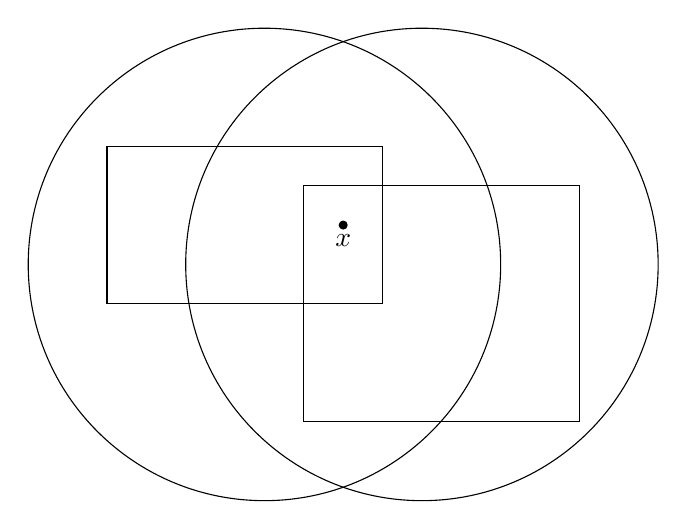
\begin{tikzpicture}
                                
                                \draw[] (-1,0) circle (3);
                                \draw[] (1,0) circle (3);
                                \draw[fill=black] (0,0.5) circle (0.05) node[below] {$x$};

                                \draw[] (-3,-0.5) rectangle (0.5, 1.5);
                                \draw[] (3,-2) rectangle (-0.5, 1);
                            \end{tikzpicture}
                        \end{center}
                        If we take the intersection of the two open rectangles, we see that we have a rectangle that surrounds the point $x$.
                        \vspace{2mm}

                        \textbf{Lemma:} The intersection of two open rectangles, if non-empty, is an open rectangle.
                        \vspace{2mm}

                        We can formalize as follows: Suppose $x\in A_1 \cap A_2$ by openness of $A_i$, there exists open rectangles $R_i$ such that $x\in R_i \subset A_i$ for $i=1,2.$ Then: 
                        \begin{equation}
                            x\in \underbrace{R_1 \cap R_2}_{\text{open rectangle}} \subset A_1 \cap A_2.
                        \end{equation}
                        To finish, we use induction. Suppose $A_i,\, i=1,\dots, n$ are open. Then: 
                        \begin{equation}
                            \bigcap_{i=1}^{n}A_i = \left(\cap_{i=1}^{n-1}A_i\right)\bigcap A_n
                        \end{equation}
                        By induction, the first part is open and by the base case, the intersection is open.
                        \vspace{2mm}

                        We can do something similar for the second part. Suppose $B_i,\, i=1,\dots, n$ is closed. Then: 
                        \begin{equation}
                            \left(\bigcup_{i=1}\right)^C = \bigcap_{i=1}^n B_i^C
                        \end{equation}
                        We've shown that the right hand side is open, so $\bigcup_{i=1}$ must be closed.
              \end{enumerate}
          \end{proof}
          \item The following is important to relate intersections and unions.
          \begin{theorem}
              \textbf{De-Morgan's Laws:} If $Y_\alpha$ is any collection of subsets of some universe $U$. Then:
              \begin{equation}
                  \left(\bigcup Y_\alpha\right)^C = \bigcap Y_\alpha^C
              \end{equation}
              and
              \begin{equation}
                  \left(\bigcap Y_\alpha\right)^C = \bigcup Y_\alpha^C
              \end{equation}
          \end{theorem}
          \item Note that part (3) of the theorem on closed/open sets is not true if we take an infinite intersection. As a counterexample, consider 
          \begin{equation}
              \bigcap_{n>0} \left(-\frac{1}{n},1+\frac{1}{n}\right) = [0,1]
          \end{equation}
          Again by De-Morgan, we can use this to construct an example of an infinite union of closed sets that is not closed.
\end{itemize}
